\pagebreak
\section{Cursograma de Ventas}
\begin{center}
 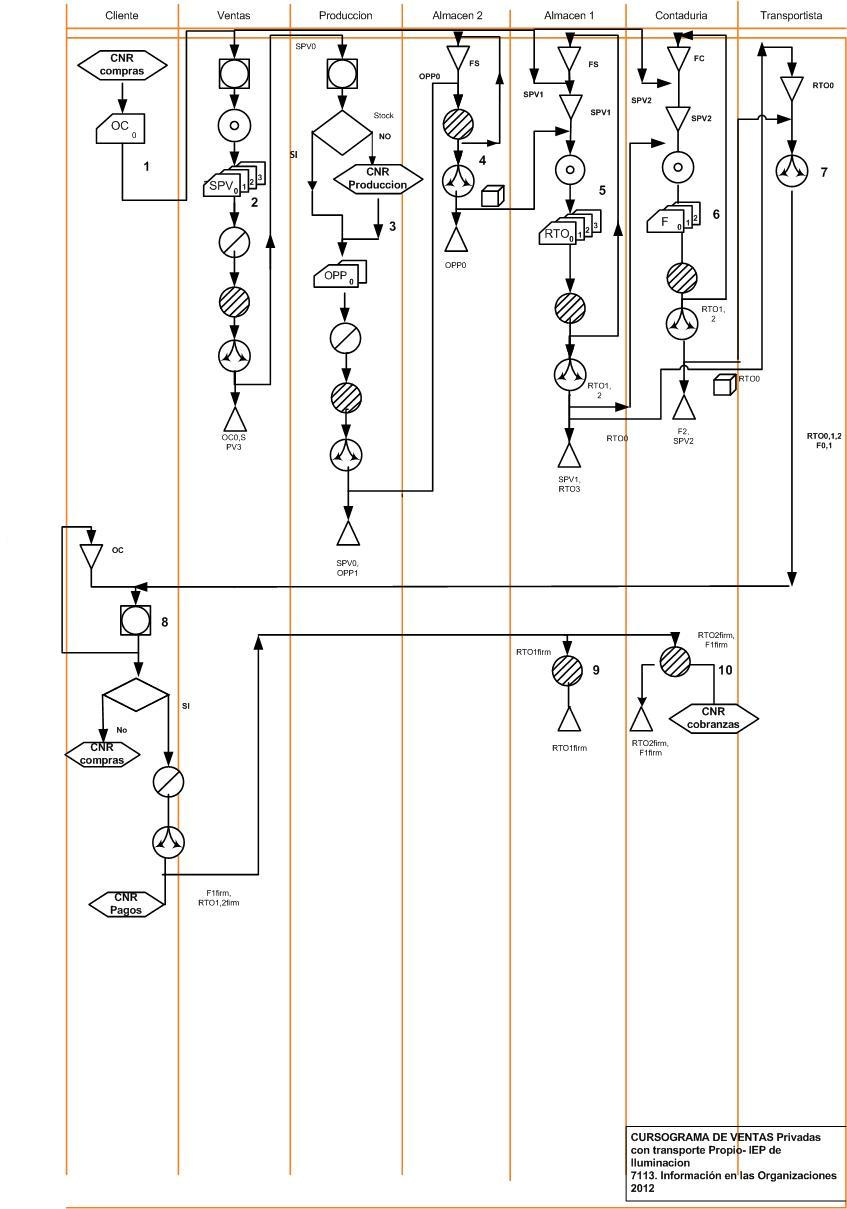
\includegraphics[scale=0.78,keepaspectratio=true]{Empresa/Circuitos/Ventas/Ventas-narrativa.jpg}
 % Ventas-narrativa.jpg: 847x1209 pixel, 96dpi, 22.41x31.99 cm, bb=0 0 635 907
\end{center}

\pagebreak
\section{Procedimiento de Ventas}
 \begin{description}
	\item[1 - Cliente] El cliente solicita un pedido emitiendo una 'Orden de Compra' (OC) mediante un 'Circuito No Relevado de Compras' (CNR Compras).
	\item[2 - Ventas] El \'area de ventas recibe la OC de parte del cliente, la controla y de esta manera genera la 'Solicitud de Pedido de Ventas' (SPV) especificando los detalles de la venta tal como est\'an especificados en la OC como por ejemplo, productos y plazo de entrega tentativo. Firma la SPV y env\'ia el original a Producci\'on y las copias a Almac\'en 1 y Contadur\'ia. Registra en el sistema la generaci\'on de la SPV y archiva en forma definitiva la 'Orden de Compra' junto a una copia de la SPV.
	\item[3 - Producci\'on] Producci\'on recibe la SPV y verifica que cuenta con stock suficiente. De no poseer stock necesario se procede a realizar el 'Circuito no relevado de de Producci\'on' (CNR Producci\'on). En caso de contar con el producto solicitado, genera una 'Orden de Pedido de Productos' (OPP) y la env\'ia a Almac\'en 2 (Almac\'en de roductos terminados).  Registra en el sistema la OPP y archiva en forma definitiva la SPV original y la copia de la OPP. 
	\item[4 - Almac\'en 2] Almac\'en 2 recibe la OPP, ya cuenta con el producto (ya sea porque ten\'ia stock o porque se ha producido especialmente) y env\'ia el producto junto con la documentaci\'on a Almac\'en 1. Registra en el sistema la actualización de la ficha de stock (FS) y el envío de productos al Almac\'en 1. Archiva definitivamente la OPP.
	\item[5 - Almac\'en 1] Almac\'en 1 prepara los productos para su entrega y genera el 'Remito' (RTO) correspondiente y tres copias. Entrega el producto al Transportista con el RTO original y entrega dos copias a Contadur\'ia. Registra en el sistema la generación de documentos y el env\'io de la mercader\'ia, y archiva en forma definitiva la 'Orden de Pedido de Productos' y una copia del Remito.
	\item[6 - Contadur\'ia] Contadur\'ia por un lado recibe la SPV asociada a la venta, y la archiva temporalmente. Al recibir el remito de Almac\'en 1 genera un listado de Remitos sin facturar asociados a la venta mediante el sistema, y emite la 'Factura'(F) correspondiente con dos copias. Registra en el sistema la emisi\'on de la factura y env\'ia el original y copia de la factura al Transportista para su env\'io al cliente. Contadur\'ia actualiza la Ficha de Cliente (FC) mediante el sistema y archiva definitivamente una copia de la factura y la SPV recibida.
	\item[7 - Transportista] Transportista recibe los remitos, las facturas y la carga a ser enviada. Env\'ia el pedido junto con la documentaci\'on al cliente. 
	\item[8 - Cliente] El cliente recibe los remitos, las facturas y el pedido. Chequea la mercader\'ia recibida junto con los documentos original, y firma las copias de los mismos. Distribuye las copias firmadas de vuelta a la empresa, y procede a realizar el 'Circuito No Relevado de Pagos' (CNR Pagos). Si la mercader\'ia no est\'a conforme a los pactado mediante la OC, se procede al CNR Compras. Conserva el Remito y Factura original.
	\item[9 - Almac\'en 1] Almacen 1 recibe la copia del remito firmado por el cliente, la registra en el sistema y lo archiva definitivamente. 
	\item[10 - Contadur\'ia] Contadur\'ia recibe la copia de la factura y el remito firmados por el cliente y la asienta la recepci\'on en el sistema. El pago de la factura es parte del 'Circuito no relevado de Cobranzas' (CNR Cobranzas)
\end{description}

\subsection{Entrevista}
Luego de analizar los diagramas de procedimiento de alto nivel del proceso de ventas que la empresa puso a nuestra disposici\'on, surgi\'o la necesidad de realizar una entrevista para aclarar ciertos puntos que no quedaban claros con nuestro contacto. Los puntos en cuesti\'on fueron los siguientes:
\begin{description}
 \item \underline{Ventas a Clientes}: \\
	Es el Centro de Atenci\'ion al Cliente (\textit{CAC}) quien interact\'ua con los clientes para realizar las ventas. Las ventas a clientes las ventas se realizan a partir de un pedido de cotizaci\'on confeccionado por el CAC. Posteriormente, el CAC formaliza el pedido de venta al recibir una Orden de Compra del cliente. Internamente, el CAC realiza una Solicitud de Pedido de Ventas (SPV).  \\
	Para el caso de los Distribuidores, ellos reciben la lista de precios y pueden formalizar directamente la Orden de Compra, es decir, que no hay cotizaci\'on previa del CAC.
 \item \underline{Registro de Clientes}: \\
	La empresa mantiene un registro de los clientes, y las transacciones que realizan con la empresa, mediante el sistema ERP Bejerman. Esta base de datos es actualizada por el \'area de Ventas, a trav\'es del \textit{CAC} y es consultada por todas las personas de la empresa que tienen habilitada esa funci\'on dentro de los m\'odulos del sistema inform\'atico. 
 \item \underline{Moviemiento de Materiales}: \\
	El medio de comunicaci\'on entre almacenes es electr\'onico, es decir, se realiza a trav\'es del sistema Bejerman, y as\'i se realizan las transferencias ``inter-dep\'osito''. Los documentos internos s\'olo se imprimen en papel cuando resulta necesario, y en casos particulares. En una \'epoca se utilizaban fichas y vale de materiales, pero fueron reemplazados por el sistema inform\'atico. Lo mismo sucede con el sector de Producci\'on, que maneja el movimiento de materiales mediante el sistema Bejerman.\\
	El sector de Producci\'on recibe por sistema la carga de datos del \'area de Ventas (CAC), formaliz\'andolo como ``Orden de Pedido''. En funci\'on a ello elabora una ``Orden de Montaje'', donde el sistema carga los elementos necesarios para confeccionar el pedido solicitado (las distintas partes y piezas para armar la luminaria). Terminado el producto, \'este se declara en el Dep\'osito Producto Terminado (02). Luego, el sector de Almacenes realiza por sistema la transferencia del producto, desde el 02 al Deposito Principal (01), y es desde aqu\'i que el \'area de Expedici\'on puede generar posteriormente el remito para despachar la mercader\'ia.  
	El transportista carga la mercader\'ia seg\'un la informaci\'on emanada de los remitos, controlando f\'isicamente la carga.  Luego se le confecciona una Hoja de Ruta con el itinerario diario y por ultimo se le emite un permiso ante el ARBA, en caso que la mercader\'ia que se transporte supere los \$20.000.-   
\end{description}

\pagebreak
\section{Cursograma de Ventas (con numeración para el manual)}
\begin{center}
 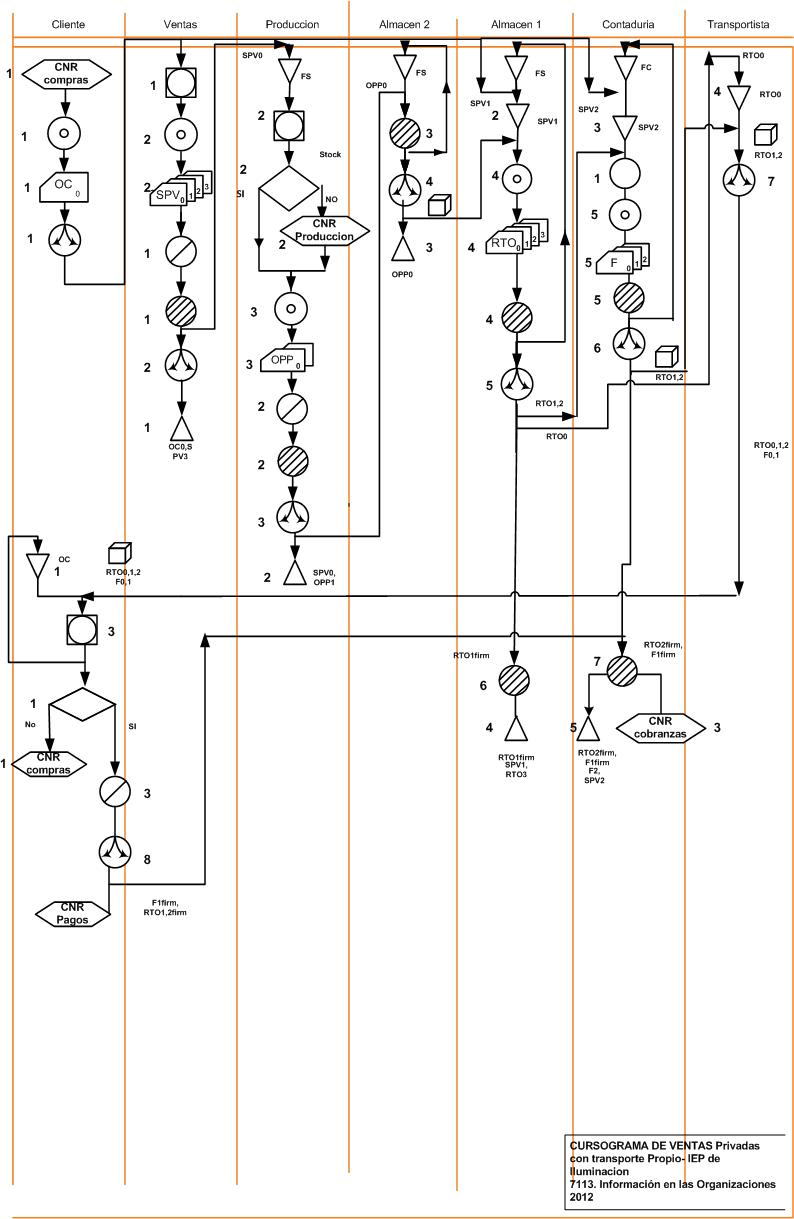
\includegraphics[scale=0.78,keepaspectratio=true]{Empresa/Circuitos/Ventas/Ventas-manual.jpg}
 % Ventas-manual.jpg: 847x1209 pixel, 96dpi, 22.41x31.99 cm, bb=0 0 635 907
\end{center}

\pagebreak
\subsection{Manual del Cursograma de Ventas}
\begin{center}\textbf{Sectores intervinientes}\end{center}
\begin{itemize}
  \item Cliente
  \item Ventas
  \item Producci\'on
  \item Almacen 2
  \item Almacen 1
  \item Contadur\'ia
  \item Transportista
\end{itemize}

\begin{center}
  \textbf{Documentos}
  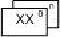
\includegraphics{./Images/Simbolos/simbolo-Documentos.png}
\end{center}
\begin{enumerate}
  \item Orden de Compra (OC).
  \item Solicitud de Pedido de Ventas (SPV).
  \item Orden de Pedido de Productos (OPP).
  \item Remito (RTO).
  \item Factura (F).
\end{enumerate}

\begin{center}
  \textbf{Emisi\'on de Documentos}
  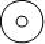
\includegraphics{./Images/Simbolos/simbolo-Emision-de-Documentos.png}
\end{center}
\begin{enumerate}
  \item Cliente emite una Orden de Compra (OC).
  \item Ventas emite una Solicitud de Pedido de Ventas (SPV) con 3 copias. 
  \item Producci\'on emite una Orden de Pedido de Productos (OPP) con duplicado.
  \item Almac\'en 1 emite Remitos (RTO) con 3 copias.
  \item Contadur\'ia emite Facturas (F) con 2 copias.
\end{enumerate}

\begin{center}
  \textbf{Firma}
  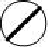
\includegraphics{./Images/Simbolos/simbolo-Firma.png}
\end{center}
\begin{enumerate}
  \item Ventas firma la Solicitud de Pedido de Ventas.
  \item Producci\'on firma la Orden de Pedido de Productos.
  \item Cliente firma las copias de remito y factura.
\end{enumerate}

\begin{center}
  \textbf{Distribuci\'on}
  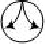
\includegraphics{./Images/Simbolos/simbolo-Distribucion.png}
\end{center}
\begin{enumerate}
  \item Cliente distribuye la OC al sector de ventas.
  \item Ventas distribuye Solicitud de Pedido de Ventas a Producci\'on, Almac\'en 1 y Contadur\'ia.
  \item Producci\'on distribuye Orden de Pedido de Productos a Almac\'en 2.
  \item Almacen 2 distribuye los productos pedidos al Almac\'en 1.
  \item Almacen 1 distribuye los Remitos junto con el pedido al Transportista.
  \item Contadur\'ia distribuye las copias de los remitos y las facturas al Trasportista.
  \item Transportista distribuye los remitos, las facturas y el pedido al Cliente.
  \item El Cliente distribuye las copias de remito y facturas firmadas a Almac\'en 1 y a Contadur\'ia.
\end{enumerate}

\begin{center}
  \textbf{Almacenamiento Transitorio}
  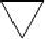
\includegraphics{./Images/Simbolos/simbolo-Almacenamiento-Transitorio.png}
\end{center}
\begin{enumerate}
  \item Cliente almacena Orden de Compra.
  \item Almac\'en 1 almacena una copia de la SPV.
  \item Contadur\'ia almacena una ficha de cliente y la SPV.
  \item Transportista almacena el remito.
\end{enumerate}

\begin{center}
  \textbf{Control y verificaci\'on}
  
\includegraphics{./Images/Simbolos/simbolo-Control-y-Verificacion.png}
\end{center}
\begin{enumerate}
	\item Ventas controla la OC recibida
	\item Producci\'on controla si cuenta con stock suficiente con la Solicitud de Pedido de Ventas.
	\item El cliente controla si el pedido recibido es realmente lo que pidi\'o con la Orden de Compra.
\end{enumerate}
\pagebreak

\begin{center}
  \textbf{Decisi\'on}
  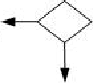
\includegraphics{./Images/Simbolos/simbolo-Decision.png}
\end{center}
\begin{enumerate}
  \item Cliente controla el pedido recibido. En caso de existir alg\'un inconveniente ejecuta parto de un 'Circuito no relevado de Compras', sino procede a la firma y distribuci\'on de los documentos firmados.
  \item Producci\'on controla el stock. De no poseer procede a realizar el 'Circuito no relevado de de Producci\'on' (CNR Producci\'on). En caso de contar con el producto solicitado, genera una 'Orden de Pedido de Productos'.

\end{enumerate}

\begin{center}
  \textbf{Registro}
  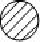
\includegraphics{./Images/Simbolos/simbolo-Registro.png}
\end{center}
\begin{enumerate}
  \item Ventas registra en el sistema la venta en curso y los documentos enviados.
  \item Producci\'on registra en el sistema la recepci\'on de la SPV y el env\'io de la OPP a Almac\'en 2.
  \item Almac\'en 2 registra en el sistema la recepci\'on de la OPP y la entrega de mercader\'ia a Almac\'en 1.
  \item Almac\'en 1 registra en el sistema la recepci\'on de la mercader\'ia la entrega de mercader\'ia.
  \item Contadur\'ia registra en el sistema la recepci\'on de SPV y los remitos, y la emisi\'on de la factura.
  \item Almac\'en 1 registra en el sistema el arribo de la copia del remito firmada por el cliente.
  \item Contadur\'ia registra en el sistema el arribo de la copia de la factura firmada por el cliente.  
\end{enumerate}

\begin{center}
  \textbf{Almacenamiento definitivo}
  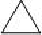
\includegraphics{./Images/Simbolos/simbolo-Almacenamiento-Definitivo.png}
\end{center}
\begin{enumerate}
  \item Ventas almacena la Orden de Compra y una copia de la SPV.
  \item Producci\'on almacena la Solicitud de Pedido de Ventas y la copia de la OPP.
  \item Almac\'en 2 almacena la OPP.
  \item Almac\'en 1 almacena la copia de la SPV, una copia del remito y la copia firmada por el cliente del remito.
  \item Contadur\'ia almacena una copia de la factura y la copia de la factura y el remito firmada por el cliente.  
\end{enumerate}

\begin{center}
  \textbf{Circuito no relevado}
  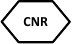
\includegraphics{./Images/Simbolos/simbolo-CNR.png}
  % simbolo-CNR.png: 73x44 pixel, 96dpi, 1.93x1.16 cm, bb=0 0 55 33
\end{center}
\begin{enumerate}
  \item Compras (circuito del cliente).
  \item Pagos (circuito del cliente).
  \item Cobranzas.
\end{enumerate}

\begin{center}
  \textbf{Documentos}
  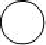
\includegraphics{./Images/Simbolos/simbolo-Operacion.png}
\end{center}
\begin{enumerate}
  \item Contaduría genera un listado remitos sin facturar asociados a la venta mediante el sistema, en base al cual arma la factura.
\end{enumerate}

\pagebreak
\section{Formularios de Ventas}

\subsection{Factura}
\begin{center}
 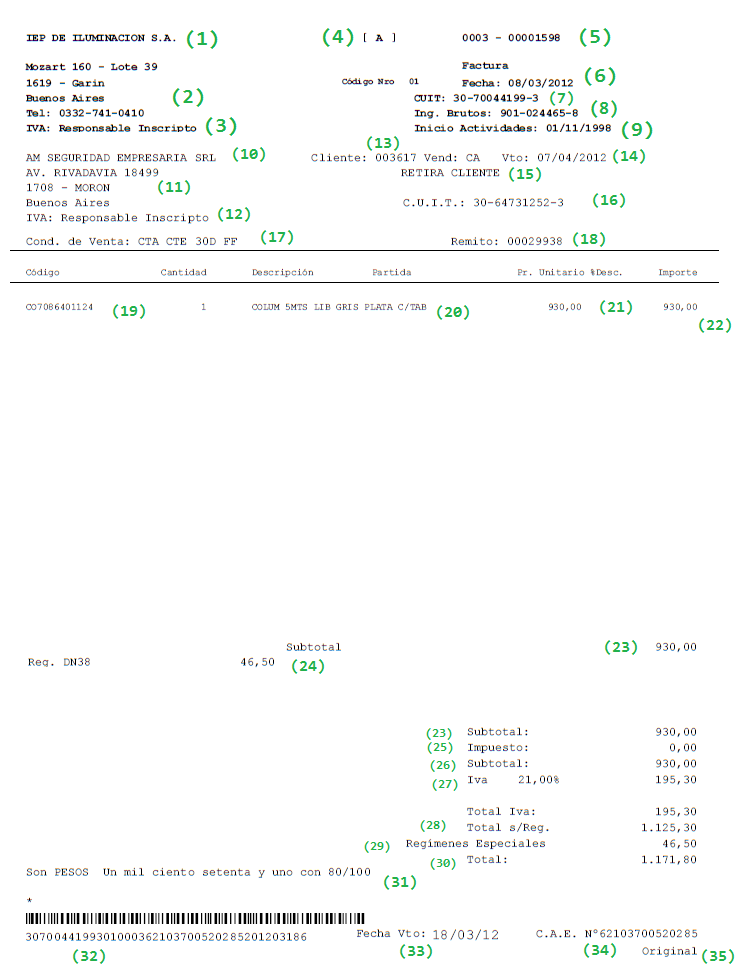
\includegraphics[scale=0.85,keepaspectratio=true]{./Images/FormulariosIEP/Factura.png}
 % Factura.png: 749x973 pixel, 96dpi, 19.82x25.75 cm, bb=0 0 562 730
\end{center}
\begin{itemize}
  \item \textbf{Objetivo:} Con este documento se notifica al cliente que efectu\'o la compra el monto total a pagar. Se especifica el remito asociado, los productos comprados con detalle de precios, los impuestos incluidos y las condiciones de pago.
  \item \textbf{Alcance:} Es un documento entre la empresa y el cliente.
  \item \textbf{Emisor:} Contadur\'ia.
  \item \textbf{Cantidad de Copias Emitidas:} Original y Copia.
  \item \textbf{Sector receptor:} Expedici\'on, para su env\'io al cliente.
\end{itemize}
\subsubsection{Descripci\'on campos de la Factura}
\begin{enumerate}
  \item Empresa emisora: Raz\'on Social de la empresa
  \item Empresa emisora: Informaci\'on de Sucursal. Domicilio y N\'umero de Tel\'efono
  \item Empresa emisora: Responsabilidad frente al IVA
  \item Tipo de Factura (A en este caso)
  \item N\'umero de Factura
  \item Fecha de emisi\'on
  \item Empresa emisora: CUIT
  \item Empresa emisora: C\'odigo de Ingresos Brutos
  \item Empresa emisora: Fecha de inicio de actividades
  \item Cliente: Raz\'on Social 
  \item Cliente: Domicilio
  \item Cliente: Responsabilidad frente al IVA
  \item C\'odigo del cliente al que se le factura y C\'odigo de Vendedor (Opcional)
  \item Vencimiento de la Factura
  \item Condici\'on de entrega
  \item Cliente: CUIT
  \item Condici\'on de Venta / Tipo de Pago.
  \item Remito asociado a la Venta.
  \item Detalle de la factura: C\'odigo interno del \'item, Cantidad del \'item
  \item Detalle de la factura: Descripci\'on del \'item. La partida asociada es opcional
  \item Detalle de la factura: Precio unitario del \'item. El descuento del \'item es opcional.
  \item Detalle de la factura: Precio total del \'item (cantidad * precio unitario)
  \item Detalle de la factura: Subtotal de items (suma de los totales de \'item)
  \item Detalle de la factura: Detalle de Reg\'imenes Especiales que aplican.
  \item Total de Impuestos que aplican a la venta (sin IVA).
  \item Subtotal con Impuestos y sin IVA.
  \item IVA discriminado.
  \item Subtotal con Impuestos e IVA, sin Reg\'imenes Especiales.
  \item Total de Reg\'imenes Especiales.
  \item Total del Importe de la Factura.
  \item Importe de la factura en palabras.(Opcional)
  \item C\'odigo de Barras de la factura. El c\'odigo tambi\'en se encuentra en forma num\'erica. 
  \item Fecha de vencimiento del C\'odigo de Impresi\'on
  \item CAE: C\'odigo de Autorizaci\'on Electr\'onico.
  \item Copia de la facura: Original, Copia, Triplicado, etc
\end{enumerate}

\subsection{Remito}
\begin{center}
 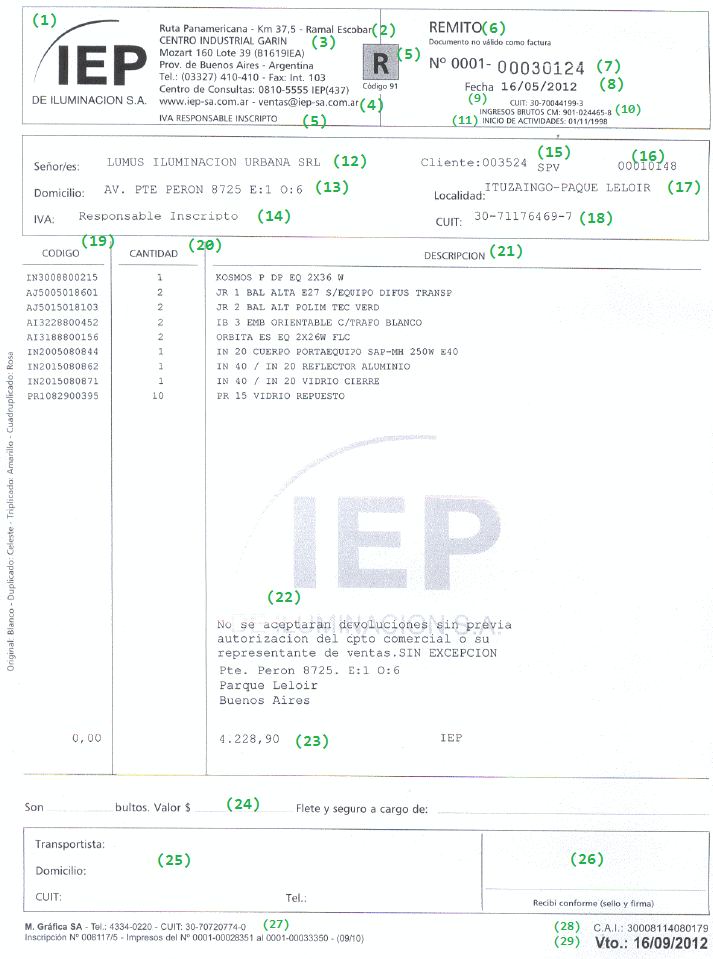
\includegraphics[scale=0.90,keepaspectratio=true]{./Images/FormulariosIEP/Remito.png}
 % Remito.png: 713x959 pixel, 96dpi, 18.87x25.38 cm, bb=0 0 535 720
\end{center}
\begin{itemize}
  \item \textbf{Objetivo:} En este documento se detallan los productos a ser enviados al cliente. No se incluyen detalles de precios y se especifica la contidad de bultos.
  \item \textbf{Alcance:} Es un documento entre la empresa y el cliente.
  \item \textbf{Emisor:} Almac\'en 1.
  \item \textbf{Cantidad de Copias Emitidas:} Original y Copia.
  \item \textbf{Sector receptor:} Expedici\'on, para su env\'io al cliente.
 \end{itemize}
\subsubsection{Descripci\'on campos del Remito}

\begin{enumerate}

   \item Empresa emisora: Logo y Raz\'on Social de la empresa
   \item Empresa emisora: Domicilio Sucursal
   \item Empresa emisora: Domicilio Legal
   \item Empresa emisora: Informaci\'on de Contacto. N\'umeros de tel\'efono, sitio web, email, fax.
   \item Empresa emisora: Responsabilidad ante el IVA
   \item Tipo de Documento: Remito (S\'imbolo).
   \item Tipo de Documento: Remito.
   \item N\'umero de Remito.
   \item Fecha de Emisi\'on del Remito
   \item Empresa emisora: CUIT
   \item Empresa emisora: C\'odigo de Ingresos Brutos.
   \item Empresa emisora: Fecha de Inicio de Actividades.
   \item Cliente: Raz\'on Social
   \item Cliente: Domicilio 
   \item Cliente: Responsabilidad ante el IVA
   \item Cliente: C\'odigo interno de Cliente
   \item Solicitud de Pedido de Venta (SPV) asociada al remito.
   \item Cliente: Localidad
   \item Cliente: CUIT
   \item Detalle del Remito: C\'odigo de Producto.
   \item Detalle del Remito: Cantidad de Producto
   \item Detalle del Remito: Descripci\'on del Producto
   \item Detalle del Remito: Nota de Condici\'on de Entrega (Opcional)
   \item Detalle del Remito: Precio Total de la Mercader\'ia
   \item Cantidad de Bultos, Precio por Bulto, Flete y Seguro (Opcionales)
   \item Transportista: Nombre o Raz\'on Social
   \item Transportista: Domicilio
   \item Transportista: CUIT y Tel\'efono
   \item Fima Del Cliente
   \item Imprenta autorizada: Tel\'efono, CUIT, N\'umero de Inscripci\'on, Rango de Remitos Impresos.
   \item Imprenta autorizada: CAI. (C\'odigo de Autorizaci\'on de Imprenta)
   \item Vencimiento del Remito.
  \end{enumerate}
  
\pagebreak
\section{Normas de Control Interno de Ventas}
\begin{itemize}
 \item	{\bf Separaci\'on de funciones: } El encargado de ventas no debe poseer acceso a las registraciones de stock ni a la modificaci\'on de cuentas del cliente.
Quien vende no puede otorgar cr\'editos ni encargarse de la facturaci\'on. Dentro del sector de Ventas existe una clara divisi\'on entre la parte encargada de la atenci\'on a los clientes 
y la parte encargada de la venta en s\'i misma.
  \item	{\bf Aprobaci\'on de la venta: } Las pol\'iticas de ventas, otorgamiento de cr\'editos y precios son dispuestas por la Direcci\'on General.
La aprobaci\'on de la venta es realizada por el responsable de cr\'editos dado que es el que conoce el estado financiero de los clientes.
  \item	{\bf Movimiento de bienes: } La circulaci\'on de mercader\'ias est\'a respaldada por comprobantes firmados por el responsable del sector que los recibe. En los sectores de Producci\'on, 
Almac\'en 1 y 2 y Expedici\'on se documenta el transpaso de mercader\'ia utilizando el correspondiente m\'odulo del sistema inform\'atico de Bejerman.
  \item	{\bf Documentaci\'on prenumerada: } Toda documantaci\'on emitida debe estar prenumerada y se archivan en orden num\'erico, incluso las anuladas. Dado que todos los documentos se generan 
utilizando el sistema inform\'atico, resulta complicado alterar la numeraci\'on dado que la misma es autogenerada utilizando una secuencia.
  \item	{\bf Control de Facturaci\'on: } Contadur\'ia realiza un control cruzado de la facturaci\'on y remitos. Contadur\'ia siempre conserva una copia de las facturas y remitos emitidos. 
A su vez, realiza un control antes de que dichos documentos sean enviados al cliente.
  \item La norma de control interno de {\bf Bonificaciones} no aplica en el caso analizado; dado que, al relevar el circuito correspondiente al \'area de ventas y consultar sobre la posibilidad de existencia 
de bonificaciones dentro del mismo, se nos mencion\'o que la empresa no trabaja de este modo, es decir, no utiliza las bonificaciones como norma de control interno.   
\end{itemize}
